%% Monografia de PCC - Desempenho das Wireless LAN
%%
\documentclass{abnt}

% Incluir Pacotes ------------------------------------------------
\usepackage[utf8]{inputenc}
\usepackage[brazil]{babel}
\usepackage{url}
%\usepackage [latin1] {inputenc}
\usepackage{ae}                         %% Font Encoding T1 (PDF)
\usepackage{graphicx}            	%% Inclusao de graficos (DVI/PS)
\usepackage{geometry}            	%% Dimensoes do documento (DVI/PS)
\usepackage{lscape}                     %% Utilizar pagina em landscape
\usepackage{url}                        %% Trata URLs, e-mails e paths
\usepackage[alf]{abntcite}
\usepackage{cite}
\usepackage{float}


%\usepackage[dvipdfm]{hyperref}% permite configurar hiperef
%\hypersetup{colorlinks=true,linkcolor=blue,citecolor=blue}

\renewcommand{\ABNTchapterfont}{\fontfamily{cmr}\fontseries{b}\selectfont}
\renewcommand{\ABNTsectionfont}{\fontfamily{cmr}\fontseries{b}}
\renewcommand{\tituloformat}{\large\bfseries}

\begin{document}
% ----------------------------------------------------------------
% Paginas iniciais
% ----------------------------------------------------------------
% ----------------------------------------------------------------
% Pginas Iniciais ***********************************************
% ----------------------------------------------------------------

% Capa -----------------------------------------------------------

\autor{
Alfredo José de Paula Barbosa - 16890 \\
Michell Stuttgart Faria - 16930 \\
Paulo Vicente Gomes dos Santos - 15993 \\
Orientador: Prof. Dr. Enzo Seraphim
}

\titulo{SAGA Game Library \\
Biblioteca para desenvolvimento \\
de jogos eletrônicos 2D \\
}

\comentario{Monografia apresentada para o Trabalho de Diploma do curso de
Engenharia da Computação da Universidade Federal de Itajubá.}

\instituicao{Universidade Federal de Itajubá - UNIFEI 
\par Instituto de Engenharia de Sistemas e Tecnologias da Informação Engenharia da
Computação}

\local{Itajubá - MG}

\data{}

\capa

\folhaderosto
                    %% Capa e Folha de rosto
\tableofcontents                  %% Sumario
\listoffigures                    %% Lista de figuras
%\listoftables                     %% Lista de tabelas
%\include{ListaAbrev}             %% Lista de abreviaturas
%\pretextualchapter{Agradecimentos}

\begin{espacosimples}
\noindent A cada mestre das nossas escolas e famílias, que nos guiaram na construção do conhecimento, dos átomos e das células, dos números e das palavras, dos fenômenos da natureza e dos mistérios da alma, da convivência, da responsabilidade e da dedicação. A cada amigo e familiar que estava lá, tanto nas lutas quanto nas vitórias, como esta, pela graça de Deus, de quem é toda a glória. 
\end{espacosimples}                 %% Agradecimentos
\begin{resumo}

Uma biblioteca de jogos ou \textit{game engine} pode ser vista como um conjunto de recursos e ferramentas para a construção de um jogo. Você pode criar um jogo sem uma biblioteca básica, assim como você pode criar uma mesa de madeira sem pregos, martelos, parafusos, chaves de fenda e serras, mas as vantagens que as ferramentas proporcionam justificam chamá-las de necessárias.
O nível dessas ferramentas varia: algumas \textit{engines} se limitam a códigos, ou seja, constantes, variáveis, funções e classes relacionadas, mas outras contam com interfaces gráficas que possibilitam o desenvolvimento de um jogo sem codificação alguma. De qualquer forma, uma \textit{game engine} precisa proporcionar, no mínimo, ferramentas para manipular sons, imagens (texto, imagens, etc), memória (dados) e controle (teclado, mouse, etc).

\vspace{1em}
\textbf{Palavras-chave}: \textit{game engine}, jogos eletrônicos, ferramentas de desenvolvimento.
\end{resumo}                 %% Resumo
%-----------------------------------------------------------------
% Corpo da Monografia
% ----------------------------------------------------------------
% ----------------------------------------------------------------
% Introdução e Conceitos Básicos *******************
% ----------------------------------------------------------------
\chapter{Introdução}
\label{cap:indtroducao}
%
Desde os primórdios da humanidade a competição é uma forma de diversão muito popular. O objetivo de qualquer competição é testar uma habilidade individual ou grupal e destacar quem ganha. Embora essa característica ainda seja a mesma, a competição está condicionada a uma evolução que pode ser notada, por exemplo, na corrida: no começo ela era individual e só testava a velocidade e a resistência da pessoa; hoje uma corrida automobilística testa a resistência, a destreza, a inteligência e a tecnologia da equipe.
Mas essa evolução não se da só na complexidade da competição, ela se manifesta da mesma forma na sua abstração. Os jogos de estratégia que nós conhecemos hoje, por exemplo, são versões abstratas das competições físicas. A aptidão física de cada criatura imaginária é determinada por alguma característica interna do jogo, porque o que o jogo de estratégia testa é o raciocínio e a estratégia da pessoa e não a sua capacidade física propriamente dita. O xadrez internacional, simulando uma guerra da Idade Média, é um caso concreto dessa evolução.
Com o avanço da microeletrônica e da computação, no entanto, o jogo de estratégia ganha uma plataforma que pode simular não só um sistema de lógica, mas toda uma realidade virtual. Qualquer jogo pode ganhar uma versão eletrônica. O jogo eletrônico, portanto, não é só uma brincadeira de criança, ele é na verdade o último estágio de um passatempo milenar. Isso se confirma pela movimentação de recursos e ganhos da indústria dos jogos eletrônicos desta geração.
%
%
% ----------------------------------------------------------------
% Motivacao *******************
% ----------------------------------------------------------------
\section{Motivação}
\label{section:motivacao}
%
%
%
Nos últimos anos, o mercado de games do Brasil tem presenciado um crescimento significativo. \cite{e}
O advento dos dispositivos móveis, como \textit{smartphones} e \textit{tablets}, e a possibilidade de comercializar seu produto \textit{online} em lojas virtuais e assim reduzir custos favoreceu, em parte, a redução da pirataria e fez com que o usuário preferisse a compra do produto original a investir em um produto não-original. Essa mudança de comportamento por parte do consumidor fez com que um mercado, que antes era visto como inseguro, passasse a ser considerado um mercado promissor pelas empresas desenvolvedoras de software, incluindo as desenvolvedoras de \textit{games}.
\par
Com o crescimento da área de desenvolvimento de jogos eletrônicos, surge também a necessidade de encontrar mão-de-obra capacitada, necessidade esta que é uma das maiores reclamações das indústrias de desenvolvimento de \textit{games} do Brasil. Por se tratar de uma área de desenvolvimento recente, é difícil encontrar profissionais capacitados na área. Uma das soluções mais simples para esta carência de mão-de-obra é incentivar estudantes, sejam eles de nível técnico ou universitário, a aprender sobre as ferramentas e técnicas mais utilizadas no desenvolvimento de um jogo eletrônico. Assim, torna-se de suma importância a implementação de ferramentas que facilitem o primeiro contato do estudante com essa complexa área de desenvolvimento, motivo este que nos motivou a criação da \textit{SAGA Game Library}.
%
%
% ----------------------------------------------------------------
% Objetivos *******************
% ----------------------------------------------------------------
\section{Objetivos}
\label{section:objetivos}
%
A \textit{SAGA Game Library} foi desenvolvida tendo em foco o meio acadêmico. Com o aumento do mercado de desenvolvimento de 
jogos eletrônicos no país, surge a necessidade de investir na capacitação de profissionais para atender a essa demanda. Não apenas profissionais do setor precisam estar em constante atualização, mas os agora estudantes e futuros profissionais também precisam de capacitação. É para esse último que é direcionada esta biblioteca de desenvolvimento. Seu objetivo primário é possibilitar ao usuário, seja ele um estudante ou entusiasta, o primeiro contato com o mundo do desenvolvimento de jogos.
%
\par
%
É certo que já existem muitas \textit{game engines}, inclusive em C++, mas o estudo é o piso de todas as descobertas científicas, o que justifica e motiva o desenvolvimento de uma biblioteca de jogos didática. Esta é a nossa proposta: uma camada de orientação a objetos envolvendo a Allegro de uma forma simples e didática. Simplicidade, eficiência e aprendizado são as palavras-chave da \textit{SAGA Game Library}.
%
%
%                   %% INTRODUCAO
% ----------------------------------------------------------------
% Revisão bibliográfica *******************
% ----------------------------------------------------------------
\chapter{Revisão Bibliográfica}
\label{cap:revisao_bibliografica}
%
%
% ----------------------------------------------------------------
% Projeto do sistema *******************
% ----------------------------------------------------------------
\section{Projeto do sistema}
%
Uma vez definidos os requisitos do sistema, a próxima etapa era dar início ao desenvolvimento do projeto. O primeiro passo foi definir, com base nos requisitos e no conhecimento dos envolvidos, qual seria a linguagem de programação mais adequada ao problema e qual API deveria ser usada para as rotinas de renderização, acesso ao dispositivos de entrada, reprodução de áudio, etc.
%
%
\subsection{Linguagem de Programação}
\label{linguagem}
%
Até a década de 90 cada jogo tinha a sua \textit{engine}, feita para possibilitar a maior eficiência no uso da memória e da unidade de processamento possível, de acordo com as exigências de cada jogo. Um jogo que só usava formas geométricas, por exemplo, não precisava tratar imagens na sua \textit{engine}. O nível da microeletrônica e da computação já possibilita o uso de \textit{engines} genéricas, mas o desenvolvimento de uma ainda demanda uma programação muito próxima da máquina. É por isso que a escolha da linguagem de programação precisa ser feita com cuidado. 
\par 
Considerando o conhecimento da equipe e o propósito do projeto, que era uma \textit{engine} didática, para influenciar o desenvolvimento de jogos de acordo com o nosso alcance, as linguagens de programação selecionadas para a análise foram Java e C++, de acordo com a simplicidade, o poder e a portabilidade de cada uma.
%
\subsubsection{Estudo Comparativo}
%
%O Actionscript é uma linguagem orientada a objetos desenvolvida pela Macromedia. O que no início era uma ferramenta para controlar animações se tornou uma linguagem de script tão complexa que podia ser usada no desenvolvimento de um jogo. Embora essa linguagem ainda seja muito usada no desenvolvimento de jogos de web, o que provocou a decisão contrária a ela foi a expectativa de que o HTML 5 viesse a incorporar o Javascript e, dessa forma, modificar ou inutilizar o Actionscript. A possibilidade de utilizar o próprio HTML 5 foi excluída porque essa versão do HTML ainda se encontra em uma fase muito incerta.
\par
%O C\# (C Sharp) é uma linguagem multi-paradigma da Microsoft feita para o desenvolvimento de sistemas próprios para a plataforma .NET. C\# e Java compartilham a mesma simplicidade na leitura e na codificação, assim como a mesma forma de interpretação e compilação, mas um programa em C\# está mais próximo da máquina do que um programa em Java. A escolha parecia feita quando nós entendemos que a ligação do C\# com a Microsoft poderia custar a portabilidade da nossa biblioteca, 
\par
Java é uma linguagem orientada a objetos desenvolvida pela Sun, hoje possuída pela Oracle. A sua fama de espaçosa e pesada não é coerente com a realidade: hoje a linguagem conta com a Compilação na Hora ou \textit{Just in Time Compilation} (\textit{JIT Compilation} ou só JIT), para que a sua execução não seja mais interpretada. Mas a sua principal característica é a portabilidade: a Máquina Virtual do Java ou Java Virtual Machine (JVM) é uma plataforma virtual compatível com a maioria das plataformas mais populares como o Microsoft Windows, Unix/Linux e MacOS X.
\par
Por mais evoluída que seja a JVM, no entanto, o Java não admite o acesso à máquina necessário para o desenvolvimento de uma \textit{game engine}, senão com o uso do C++, por meio da Interface Nativa do Java ou Java Native Interface (JNI). Em outras palavras, para usar o Java, nesse caso, nós teríamos que usar o C++. Esta, por sua vez, não é a mais simples na codificação, mas não tem limitação alguma tanto em termos de portabilidade, pois conta com um padrão oficial e compiladores para várias plataformas, quanto em termos de acesso à máquina.
%
%\subsubsection{A Escolha: C++}
%
\par
C++ (C Mais Mais ou C Plus Plus) é uma linguagem de programação multi-paradigma, com suporte para a programação imperativa e a programação orientada a objetos, de uso geral, desenvolvida por Bjarne Stroustrup, para formar uma camada de orientação a objetos sobre a linguagem de programação C. O C++ possibilita a programação de baixo nível assim como a programação de alto nível e por isso é considerado uma linguagem de programação de nível médio em termos de proximidade da máquina \cite{Mizrahi} .
\par
Após o estudo comparativo, concluímos que a linguagem C++ seria a melhor opção para o projeto em questão. Tal decisão foi baseada em diversos fatores, como experiência e domínio da linguagem pelos envolvidos no projeto, o desempenho das aplicações escritas nesta linguagem e o fato de C++ ser a linguagem de programação mais usada no desenvolvimento de jogos. Uma vez que o objetivo da biblioteca é ser uma porta de entrada para essa área, a escolha da linguagem faz com que o usuário já se familiarize com a mesma. %Por último e não menos importante, o C++ é uma linguagem 100\% compatível com a API escolhida como base para a nossa \textit{engine} que será abordada a seguir.
%
%
\subsection{Allegro}
\label{allegro}
%
Nas nossas pesquisas para escolher uma biblioteca com a qual trabalhar, duas se destacaram: a Allegro e a SDL. A SDL (\textit{Simple Direct Media Layer} ou \textit{Camada de Mídia Direta Simples}) é uma biblioteca multimídia simples de usar, multiplataforma, de código aberto, e amplamente usada para fazer jogos e aplicações multimídia \cite{SDLDoc}. Ela também poderia atender às nossas necessidades, mas a Allegro se destacou por ter um código mais limpo e intuitivo, e rotinas específicas para o desenvolvimento de jogos, como renderização acelerada por hardware e suporte nativos a diversos formatos de imagens e arquivos de áudio. Por esta razão ela foi escolhida.
\par 
Allegro é uma biblioteca gráfica multiplataforma, de código fonte aberto e feita na sua maioria em C, mas utilizando internamente também Assembly e C++. Seu nome é um acrônimo recursivo que representa ``\textit{Allegro Low Level Game Routines}'' (``Rotinas de jogo de baixo nível Allegro''). Funciona em diversos compiladores e possui rotinas para a manipulação de funções multimídia de um computador, além de oferecer um ambiente ideal para o desenvolvimento de jogos, tornando-se uma das mais populares ferramentas para esse fim atualmente. Originalmente desenvolvida por Shawn Hargreaves, ela se tornou um projeto colaborativo, com colaboradores de todo o mundo \cite{AllegroDoc}.
\par
Ela possui suporte nativo para rotinas de que utilizam gráficos 2D, embora seja possível utilizá-la em conjuntos com outras APIs, como OpenGL e DirectX, para desenvolvimento de aplicações que utilizem gráficos 3D. Apesar de não ser suficiente para o completo desenvolvimento de um jogo, existem pequenas bibliotecas adicionais (\textit{add-ons}), feitas para serem acopladas à Allegro, permitindo assim a sua extensão. Através desses \textit{add-ons} é possível, por exemplo, obter suporte a arquivos MP3, GIF, imagens JPG e vídeos AVI \cite{AllegroDoc}. %Isso é útil para que o usuário não tenha que colocar uma porção de funções que não usa na hora de distribuir seu jogo, incluindo somente as partes que for utilizar, diminuindo consideravelmente o tamanho do mesmo \cite{AllegroDoc}.
\par
Atualmente, a biblioteca se encontra na sua quinta versão. Allegro 5 foi completamente reescrita e não apresenta compatibilidade com as suas versões anteriores. Foi feito um esforço para tornar a API mais consistente e segura, o que trouxe melhorias funcionais e uma grande mudança na sua arquitetura, sendo agora orientada a eventos e possuindo suporte nativo a aceleração por hardware. Possui suporte a eventos gerados por dispositivos de entradas como teclado, \textit{mouse} e \textit{joystick} além de funções para desenho de primitivas gráficas, leitura e gravação de seu próprio tipo de arquivo de configuração (muito útil para armazenar configurações e dados de jogos) e é totalmente modular \cite{AllegroDoc}.
\par
A Allegro 5.0 suporta as seguintes plataformas:
%
\begin{itemize}
 \item Windows (MSVC, MinGW);
 \item Unix/Linux;
 \item MacOS X;
 \item iPhone;
 \item Android (Suporte provido pela Allegro 5.1, que ainda se encontra instável).
\end{itemize}
%
A API atualmente se encontra nas versões 5.0.10 (estável) e 5.1.2 (instável). A \textit{SAGA Game Library} foi desenvolvida usando como base a versão 5.0.10.
%10
\subsubsection{Características Técnicas}
%
Uma vez que a Allegro é codificada na sua maioria em C, a principal característica dessa biblioteca é a estrutura imperativa. Embora algumas funções internas usem outras técnicas, a interface da Allegro é completamente imperativa, o que determina que a programação de qualquer jogo desenvolvido nessa biblioteca seja imperativa ou híbrida, a não ser que ela própria seja encapsulada.
\par
Outra característica da Allegro, profundamente relacionada com a linguagem C, é o uso de ponteiros, o que torna a codificação complicada e consequentemente propícia a erros, e a execução ligeiramente mais lenta. Esses detalhes exigem um cuidado especial no processo de encapsulamento da Allegro.
%
\subsubsection{Principais Recursos e Funções}
%
A seguir, encontramos um conjunto dos principais recursos da Allegro 5, começando com as funções mais gerais da biblioteca \cite{AllegroDoc}.
%
\begin{itemize}
 \item \textbf{al\_init()}: Inicializa a biblioteca Allegro, dando valores a algumas variáveis globais e reservando memória. 
 Deve ser a primeira função a ser chamada.
 \item \textbf{al\_exit()}: Encerra a Allegro. Isto inclui retornar ao modo texto e remover qualquer rotina que tenha sido instalada. 
 Não há necessidade de chamar essa função explicitamente, pois, normalmente, isto é feito quando o programa termina.
\end{itemize}
%
As rotinas de vídeo:
%
\begin{itemize}
 \item \textbf{ALLEGRO\_DISPLAY}: Tipo que representa a janela principal. A biblioteca permite que se trabalhe com múltiplas janelas.
 \item \textbf{al\_create\_display(width, height)}: Cria uma instância da janela, retornando um ponteiro para ALLEGRO\_DISPLAY. 
 Os parâmetros indicam as dimensões em pixels.
 \item \textbf{al\_flip\_display()}: Função para atualizar a tela.
 \item \textbf{al\_destroy\_display(var)}: Finaliza a instância \textit{var} do tipo ALLEGRO\_DISPLAY\*.
\end{itemize}
%
As rotinas para manipulação de arquivos de imagem:
%
\begin{itemize}
 \item \textbf{ALLEGRO\_BITMAP}: Tipo que representa o arquivo de imagem carregado pela Allegro.
 \item \textbf{al\_init\_image\_addon()}: Inicializa o add-on da Allegro 5 para utilização de imagens.
 \item \textbf{al\_load\_bitmap(``example.jpg'')}: Carrega a imagem indicando no parâmetro o nome e tipo. Ela deve estar previamente salva na pasta 
 do programa. Recebe o caminho relativo ou absoluto da imagem a ser carregada, retornando um ponteiro para o tipo ALLEGRO\_BITMAP.
 \item \textbf{al\_draw\_bitmap(bitmap, x, y, mirror)}: Função para desenhar a imagem na tela. Os parâmetros são o bitmap a ser desenhado, as 
 posições x e y e as flags de espelhamento (0, ALLEGRO\_FLIP\_HORIZONTAL, ALLEGRO\_FLIP\_VERTICAL).
\end{itemize}
% 
As rotinas de áudio:
%
\begin{itemize}
 \item \textbf{ALLEGRO\_SAMPLE}: Tipo que representa arquivos pequenos, geralmente efeitos sonoros.
 \item \textbf{ALLEGRO\_AUDIO\_STREAM}: Tipo para representar arquivos grandes, de forma que o arquivo não é carregado de uma vez para a 
 memória. Geralmente representa os arquivos que irão compor uma trilha sonora.
 \item \textbf{al\_install\_audio()} e \textbf{al\_init\_acodec\_addon()}: A primeira inicializa as funções relativas ao áudio. A segunda inicializa os 
 codecs necessários para carregar os diversos formatos de arquivo suportados. Fornece suporte a alguns formatos, como Ogg, Flac e Wave.
 \item \textbf{al\_set\_audio\_stream\_playing(musica, true)}: Função que recebe o arquivo de áudio já carregado no primeiro parâmetro e um tipo 
 booleano no segundo (true para fazê-la tocar ou false, em caso contrário).
 \item \textbf{al\_destroy\_audio\_stream(musica) } e \textbf{al\_destroy\_sample(sample)}: Funções de desalocação dos arquivo de áudio carregados 
 pela Allegro.
\end{itemize}
%
%
A Allegro ainda possui muitos recursos que não foram citados devido a sua quantidade. Posteriormente, a API será explorada mais a fundo conforme os recursos da \textit{SAGA Game Library} forem mostrados.
%
%

\subsection{Suporte ao Tiled}
%
A edição de níveis ou cenários é uma das tarefas mais complexas no desenvolvimento de um jogo. Todo o processo, desde a elaboração artística do cenário até a maneira como o jogador irá interagir com o mesmo, exige muito planejamento e demanda muito esforço em sua implementação. Com o objetivo de facilitar esse trabalho, surgiram os editores de níveis. 
\par
Os editores de níveis são \textit{softwares} destinados à construção de cenários em jogos, o que faz deles ferramentas de grande importância para uma \textit{game engine}. Neste ponto, existem duas opções disponíveis para quem deseja implementar uma \textit{engine}: desenvolver seu próprio editor ou utilizar um editor externo, desenvolvido por terceiros. Desenvolver um editor próprio demanda muito estudo e tempo de desenvolvimento, além do que já é necessário para implementar a \textit{engine}. Tendo isso em mente, chegou-se à conclusão de que o melhor seria oferecer suporte a um editor externo, no que o editor Tiled foi escolhido. 
\par
O software Tiled, cuja interface pode ser visualizada na Figura \ref{tiledGUI}, é uma ferramenta gratuita desenvolvida em C++ para a criação de \textit{layouts} e mapas usando \textit{tilesets}, baseado na técnica de \textit{Tilemap}. Ele suporta mapas com projeções ortogonais e isométricas e ainda permite que objetos personalizados sejam salvos como imagens na resolução que se desejar. Tem suporte também a comandos externos, \textit{plugins} e formatos usados por outros editores \cite{SiteTiled}.
%
\begin{figure}[H]
    \centering
     \caption{Detalhes da interface do Tiled.}
    \label{tiledGUI}
    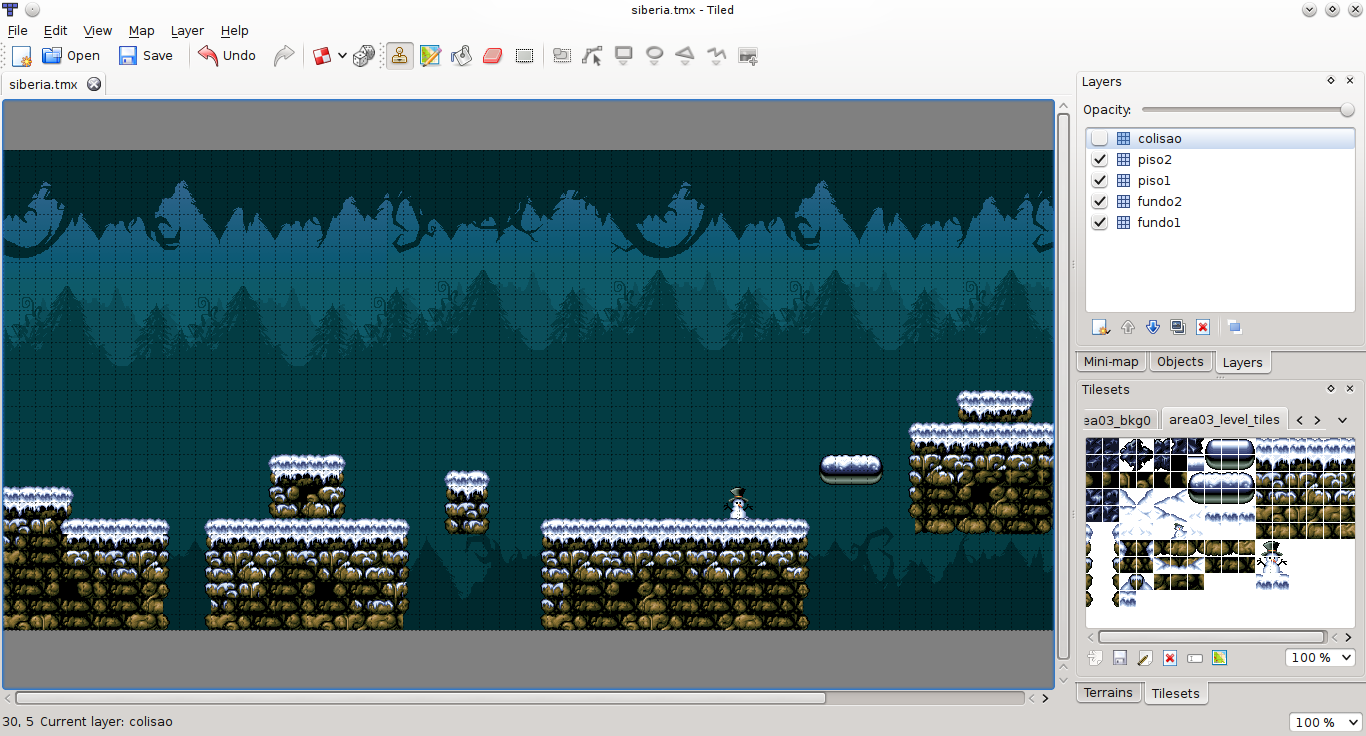
\includegraphics[scale = 0.45]{Imagens/Tiled.png}
    \\Fonte: \textit{Printscreen} da aplicação no sistema operacional Linux Mint.
\end{figure}
%
%Mesmo que o desenvolvedor não queira que seu jogo seja baseado em \textit{tiles}, o \textit{software} é ainda uma excelente escolha como um editor de níveis. Pode-se usá-lo também nas entidades invisíveis, tais como áreas de colisão e o aparecimento de objetos dentro do mapa. 
%
%\subsection{Suporte ao Tiled}
%
\par
O Tiled faz a edição de várias camadas de \textit{tiles} e salva tudo em um formato padronizado de extensão ``.tmx''. Uma das principais vantagens do formato TMX é sua organização, detalhamento e praticidade, sendo que seu conteúdo pode ser lido através do uso de um \textit{parser} para arquivos XML. XML (\textit{Extensible Markup Language} ou \textit{Linguagem de Marcação Extensível}) é um formato de texto simples e flexível que permite a criação de documentos contendo dados organizados de maneira hierárquica \cite{XMLDOC}.  
% \par 
% Existem inúmeros \textit{parsers} de arquivos XML, cada um com suas vantagens e desvantagens. Entre os \textit{parsers} mais populares podemos citar a RapidXML e a TinyXML. Segundos comparação do próprio desenvolvedor, a RapidXML apresenta a maior velocidade da leitura de dados entre os \textit{parsers} mais populares, mas o escolhido foi a TinyXML, por sua simplicidade de uso e velocidade que não apresenta uma diferença significativa a sua concorrente RapidXML. 
%
%
\subsubsection{A biblioteca TinyXML}
\label{tinyXML}
%
É uma biblioteca escrita em C++, que analisa uma sequência de entrada no formato XML, permitindo o acesso aos dados contidos nesse último. Em outras palavras, ela realiza o \textit{parsering} de uma arquivo .xml e armazena a informação em objetos C++ que podem ser manipulados livremente. Ela pode ser facilmente integrada em outros programas, bastando apenas adicionar seus arquivos ao projeto. Com ela é possível realizar o acesso aos dados direta ou iterativamente, a alteração da estrutura através de inserção e remoção de elementos, a remoção de espaços duplicados e a gravação para ficheiros em formato XML \cite{TinyXMLTutorial}.
\par
TinyXML é uma estrutura extremamente compacta e robusta, elaborada para um rápido e fácil aprendizado. Pode ser usada para fins de código aberto ou comerciais. Ela é compatível com UTF-8, de modo a permitir que arquivos XML sejam manipulados em qualquer linguagem humana. Também apresenta grande simplicidade em seu uso e rapidez na leitura de dados \cite{TinyXMLTutorial}. Devido a essas características, a TinyXML foi escolhida para realizar o \textit{parsering} dos arquivos .tmx gerados pelo Tiles.
%
%
\subsubsection{Tiled: Codificação e compactação de dados}
%
%
Um dos recursos mais interessantes do Tiled é a possibilidade de exportar os dados contidos no arquivo .tmx de forma compactada e codificada. A principal vantagem do uso dos algoritmos compactação e codificação é a redução do tamanho em disco do arquivo .tmx resultante e o aumento da velocidade de carregamento do cenário, uma vez que a biblioteca carrega os dados codificados e/ou compactados e os decodifica/descompacta a nível de software, ao invés de realizar a leitura dos mesmo em disco. 
\par 
A compactação de dados fornecida pelo Tiled é realizada pelas bibliotecas ZLIB \footnote{ZLIB: http://www.zlib.net/} e GZIP \footnote{GZIP: http://www.gnu.org/software/gzip/gzip.html}, enquanto a codificação é realizada pelo algoritmo Base64 \footnote{Algoritmo Base64: http://www.adp-gmbh.ch/cpp/common/base64.html}, também fornecido por uma biblioteca externa. São fornecidas as opções de exportar os dados no arquivo .tmx na forma codificada e compactada ou apenas na forma codificada. Também são oferecidas as opções de exportar os dados em formato puro (sem codificação) XML ou no formato CSV (\textit{Comma Separated Value} ou \textit{Valores Separados por Vírgula}), que consiste simplesmente em um arquivo de texto onde os dados são separados por vírgulas \footnote{CSV: http://creativyst.com/Doc/Articles/CSV/CSV01.htm\#FileFormat}. 
\par 
A \textit{SAGA Game Library} provê suporte às 5 opções de exportação acima. Ela, assim como o Tiled, também faz uso das bibliotecas GZIP e ZLIB para descompactação e também realiza a decodificação dos dados em Base64 contidos no arquivo .tmx (detalhes de uso serão abordados posteriormente).
%
%
%
%
% ----------------------------------------------------------------
% Implementação *******************
% ----------------------------------------------------------------

                   %% Como escrever um projeto de pesquisa
\chapter{Conclusão}
\label{conclusao}
%
Através deste projeto, nós concluímos que o desenvolvimento de jogos eletrônicos, em toda a sua extensão, envolve várias habilidades importantes para qualquer profissão da área da tecnologia, como a criatividade e a lógica matemática, especialmente para a tecnologia da informação e a engenharia da computação, como as técnicas de programação e a engenharia de software, o que confirma a viabilidade do uso dessa atividade de uma forma didática.

Ainda mais considerando a tendência da inclusão de disciplinas de programação na grade do ensino fundamental \nocite{OLHARDIG}, em qual contexto essa atividade seria um grande incentivo, senão no mínimo um meio de divulgação da programação, que por sua vez colaboraria com a educação de uma forma geral. Por mais utópica que pareça, essa expectativa está de acordo com a nossa realidade -- o Brasil é o quarto maior consumidor de games do mundo \nocite{ESTADAO}. 
\par 
O projeto nos proporcionou um rico aprendizado sobre a área de desenvolvimento de jogos eletrônicos, bem como das técnicas utilizadas no desenvolvimento e na programação dos mesmos. Por meio de pesquisa e dedicação, conseguimos implementar um \textit{software} que foi ao encontro de todos os requisitos estipulados no inicio do projeto. Uma vez que a \textit{SAGA Game Library} esteja finalizada e totalmente testada, pretendemos torná-la um projeto de \textit{software} livre, de modo que tanto escolas e estudantes quanto entusiastas possam utilizá-la para projetos educacionais, pessoais ou até mesmo comerciais.
% ----------------------------------------------------------------
\bibliographystyle{abnt-alf}
\bibliography{biblio}             %% REFERENCIAS (deve-se possuir o arquivo do tipo bibitex)
% ----------------------------------------------------------------
\end{document}
% ----------------------------------------------------------------
